%# -*- coding:utf-8 -*-
\chapter[基于张量优化的鲁棒无监督特征提取:$\ell_{1}$与$\ell_{\infty}$方法]{基于张量优化的鲁棒无监督特征提取:\\$\ell_{1}$与$\ell_{\infty}$方法}\label{chap:linf}
\echapter{Tensor Optimization-Based Robust Unsupervised Feature Extraction: The $\ell_{1}$ and $\ell_{\infty}$ Methods}

本章将介绍基于张量优化的鲁棒无监督特征提取方法——$\ell_{1}$与$\ell_{\infty}$方法。本章将首先给出$\ell_{1}$方法的优化模型。随后,本章将为$\ell_{1}$方法设计一种有效的优化算法,并从理论上分析优化算法的收敛性与计算复杂度。之后,本章将给出$\ell_{\infty}$方法的优化模型,并为之设计一种有效的优化算法。由于最终得到的$\ell_{\infty}$方法的优化算法与$\ell_{1}$方法的优化算法仅有微小差异,故本章将基于$\ell_{1}$方法的优化算法的理论收敛性分析与计算复杂度分析简要阐述$\ell_{\infty}$方法的相应理论分析结果。$\ell_{1}$与$\ell_{\infty}$方法的流程如\reffig{fig:l1linf-routine}所示。

\begin{figure}[!ht]
	\centering
    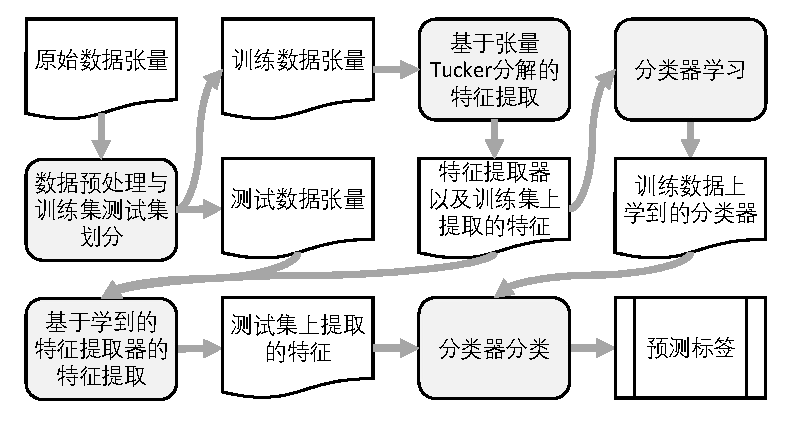
\includegraphics[width=.8\linewidth]{figures/pipeline-ufe.pdf}
	\caption{$\ell_{1}$与$\ell_{\infty}$方法的流程示意图}
	\label{fig:l1linf-routine}
\end{figure}

\section{$\ell_{1}$方法的优化模型与优化算法}
\esection{The Optimization Model and Optimization Algorithm of the $\ell_{1}$ Method}
本节将首先给出$\ell_{1}$方法的优化模型,并分析其利弊。之后,本节将设计一种用于求解$\ell_{1}$方法的有效优化算法,并对该算法进行理论上的收敛性分析以及计算复杂度分析。
\subsection{$\ell_{1}$方法的优化模型}\label{sec:l1}
\esubsection{The Optimization Model of the $\ell_{1}$ Method}
如\refsection{sec:l2}所述,$\ell_2$方法由于目标函数平滑,因此相对容易求解。但是,在实际应用场景中数据往往存在噪声与离群点,而$\ell_2$方法对它们敏感,因而并不鲁棒。这将直接影响到被提取的特征的质量。为了从带噪声与离群点的数据中更加有效地提取特征,受到机器学习理论\ucite{Goodfellow2016}与相关工作的启发,本节提出了基于$\ell_{1}$范数的非负张量Tucker分解方法(简称$\ell_{1}$方法)以提升在噪声场景下的特征提取的鲁棒性。与$\ell_{2}$方法(即\refopt{eq:L2})类似,$\ell_{1}$方法的优化模型为
\begin{equation}\label{eq:L1}
\hspace{1em}
    \begin{aligned}
    &\underset{\mathclap{\{\mathbfcal{G}^{(i)}\}_{i=1}^{n}, \{\boldsymbol{A}^{(j)}\}_{j=1}^{d}}}{\min} \qquad\quad &&\sum_{k=1}^{n}\left\|\mathbfcal{X}^{(k)}-\mathbfcal{G}^{(k)} \times_{1} \boldsymbol{A}^{(1)} \times_{2} \boldsymbol{A}^{(2)} \times_{3} \ldots \times_{d} \boldsymbol{A}^{(d)}\right\|_{F} \\
    &\text{s.t.} && \mathbfcal{G}^{(i)}\in\mathbb{R}_{+}^{r_1 \times r_2 \times \ldots \times r_d},~\forall~i\in[n] ,~\boldsymbol{A}^{(j)}\in \mathbb{R}_{+}^{n_j \times r_j},~\forall~j\in[d],
    \end{aligned}
\end{equation}
其中各符号的意义与\refsection{sec:l2}中相同,这里不再赘述。与$\ell_{2}$方法相异,$\ell_{1}$方法直接计算所有样本Tucker分解拟合误差之和作为其目标函数,因而具备更好的抗噪性能\ucite{Goodfellow2016}。然而,尽管如此,
% 可以在一定程度上抑制数据中的噪声与离群点所带来的负面影响,但其
$\ell_{1}$方法分配给不同样本的权重仍然是相同的,而这正是$\ell_{1}$方法不太合理的地方。直观上来讲,应该更关注于那些具有更大拟合误差的样本,因为一旦控制住了它们的拟合误差,那么最坏情况下的特征提取效用也就得到了保证。此外,由于\refopt{eq:L1}的目标函数是非光滑的,它的求解将会是难题。下一节将设计一种有效的优化算法来求解这个优化难题。

\subsection{优化算法设计}\label{sec:l1-algodesign}
\esubsection{Design of the Optimization Algorithm}
基于迭代优化的思想,本节设计一种用于求解\refopt{eq:L1}的有效迭代优化算法。本节接下来依次推导各个优化变量的更新公式。

\textbf{$\{\mathbfcal{G}^{(i)}\}_{i=1}^{n}$的更新:}固定$i\in[n]$,仅与$\mathbfcal{G}^{(i)}$有关的子问题如下
\begin{equation*}
    \begin{aligned}
    &\underset{\mathclap{\mathbfcal{G}^{(i)}}}{\min} &&\left\|\mathbfcal{X}^{(i)}-\mathbfcal{G}^{(i)} \times_{1} \boldsymbol{A}^{(1)} \times_{2} \boldsymbol{A}^{(2)} \times_{3} \ldots \times_{d} \boldsymbol{A}^{(d)}\right\|_{F} \\
    &\text{s.t.} && \mathbfcal{G}^{(i)}\in\mathbb{R}_{+}^{r_1 \times r_2 \times \ldots \times r_d}.
    \end{aligned}
\end{equation*}
通过简单的平方技巧,上述优化问题等价于如下更容易求解的光滑优化问题
\begin{equation*}
\begin{aligned}
    &\underset{{\mathbfcal{G}^{(i)}}}{\min} && \left\|\mathbfcal{X}^{(i)}-\mathbfcal{G}^{(i)} \times_{1} \boldsymbol{A}^{(1)}\times_{2} \boldsymbol{A}^{(2)}\times_{3}  \ldots \times_{d} \boldsymbol{A}^{(d)}\right\|_{F}^2 \\ &\text{s.t.} && \mathbfcal{G}^{(i)}\in\mathbb{R}_{+}^{r_1 \times r_2 \times \ldots \times r_d}.
\end{aligned}
\end{equation*}
由于以上优化问题对不同的$i=1,2,\ldots,n$均具有相同的形式,因而可以将它们垛叠起来一并分析,即如下优化问题
\begin{equation*}
\begin{aligned}
    &\underset{\mathbfcal{G}}{\min}&& \left\|\mathbfcal{X}-\mathbfcal{G} \times_{1} \boldsymbol{A}^{(1)} \times_{2} \boldsymbol{A}^{(2)}\times_{3} \ldots \times_{d} \boldsymbol{A}^{(d)}\right\|_{F}^2 \\ &\text{s.t.}&& \mathbfcal{G}\in\mathbb{R}_{+}^{r_1 \times r_2 \times \ldots \times r_d \times n},
\end{aligned}
\end{equation*}
其中$\mathbfcal{G}$由$\mathbfcal{G}^{(i)}$垛叠而成。由于该问题是标准的非负张量Tucker分解问题,因此可以直接应用文献\ucite{nnegTucker}中介绍的算法更新之(该算法的本质仍为非负矩阵分解的Lee-Seung算法\ucite{lee2001algorithms}),即
\begin{equation}\label{eq:l1-updateG}
	\mathbfcal{G} \leftarrow \mathbfcal{G} \oast \frac{\mathbfcal{X} \times_{1} {\boldsymbol{A}^{(1)}}^{\top}\times_{2} {\boldsymbol{A}^{(2)}}^{\top}\times_{3}  \ldots \times_{d} {\boldsymbol{A}^{(d)}}^{\top}}
	{\mathbfcal{G} \times_{1} {\boldsymbol{A}^{(1)}}^{\top} \boldsymbol{A}^{(1)} \times_{2} {\boldsymbol{A}^{(2)}}^{\top} \boldsymbol{A}^{(2)} \times_{3}  \ldots \times_{d} {\boldsymbol{A}^{(d)}}^{\top} \boldsymbol{A}^{(d)}}.
\end{equation}
% \ucite{nnegTucker}

\textbf{$\{\boldsymbol{A}^{(j)}\}_{j=1}^{d}$的更新:}固定$j\in[d]$,仅与$\boldsymbol{A}^{(j)}$有关的子问题如下
\begin{equation*}
% \hspace{-0.5em}
\begin{aligned}
    &\underset{\boldsymbol{A}^{(j)}}{\min}\qquad&& \sum_{k=1}^{n}\left\|\mathbfcal{X}^{(k)}-\mathbfcal{G}^{(k)} \times_{1} \boldsymbol{A}^{(1)} \times_{2} \boldsymbol{A}^{(2)}\times_{3}\ldots \times_{d} \boldsymbol{A}^{(d)}\right\|_{F} \\ &\text{s.t. }&& \boldsymbol{A}^{(j)}\in \mathbb{R}_{+}^{n_j \times r_j}.
\end{aligned}
\end{equation*}
利用\refsection{sec:tensor-decomp}中介绍的mode-$j$展开技巧,上述优化问题可以被等价为其矩阵形式,即
\begin{equation}\label{eq:l1-socp}
\begin{aligned}
    &\underset{\boldsymbol{A}^{(j)}}{\min}\qquad&& \sum_{k=1}^{n}\left\|\boldsymbol{X}^{(k)}_{(j)}  - \boldsymbol{A}^{(j)} \boldsymbol{G}^{(k)}_{(j)} {\boldsymbol{A}^{(\setminus j)}}^{\top} \right\|_{F} \\ &\text{s.t. }&& \boldsymbol{A}^{(j)}\in \mathbb{R}_{+}^{n_j \times r_j},
\end{aligned}
\end{equation}
其中
\begin{equation*}
    \boldsymbol{A}^{(\setminus j)} := \boldsymbol{A}^{(d)} \otimes \ldots \otimes \boldsymbol{A}^{(j+1)} \otimes \boldsymbol{A}^{(j-1)} \otimes \ldots \otimes \boldsymbol{A}^{(1)}.
\end{equation*}
更进一步地,以上优化问题可以被再次等价为如下优化问题
\begin{equation*}
    \begin{aligned}
    &\underset{\mathclap{\boldsymbol{A}^{(j)},\boldsymbol{q}}}{\min} && \boldsymbol{q}^{\top}\boldsymbol{1}_{n} \\
    &\text{s.t.} && \left\|\boldsymbol{X}^{(k)}_{(j)}- \boldsymbol{A}^{(j)} \boldsymbol{G}^{(k)}_{(j)} {\boldsymbol{A}^{(\setminus j)}}^{\top}\right\|_{F} \leq q_{k},~\forall~ k\in[n],~\boldsymbol{A}^{(j)} \in \mathbb{R}_{+}^{n_j \times r_j}.
    \end{aligned}
\end{equation*}
变换到这一步时,$\boldsymbol{A}^{(j)}$子问题其实就已经被解决了。这是因为上述优化问题为二阶锥规划问题\ucite{alizadeh2003second},而二阶锥规划为凸优化问题\ucite{boyd2004convex}。这个问题已经在业内被广泛研究与应用,并且已经有许多成熟的凸优化求解器可以快速求解。本文将使用求解器MOSEK\footnote{\url{https://www.mosek.com/}}来求解上述优化问题。

用于求解$\ell_1$方法的优化算法如\refalg{alg:l1}所示。具体来说,\refalg{alg:l1}首先初始化核心张量与因子矩阵(第1行)。之后,\refalg{alg:l1}使用\refequation{eq:l1-updateG}来更新核心张量$\mathbfcal{G}$(第4行),并通过使用MOSEK求解一系列二阶锥规划问题的方式来更新因子矩阵$\{\boldsymbol{A}^{(j)}\}_{j=1}^{d}$(第5-6行)。在达到某些收敛条件时,\refalg{alg:l1}将停止迭代,并返回学习得到的特征提取器$\{\boldsymbol{A}^{(j)}\}_{j=1}^{d}$(第9行)。

\begin{algorithm}[t]\setstretch{1.35}
	\begin{algorithmic}[1]
	\REQUIRE 张量$\mathbfcal{X} \in \mathbb{R}_{+}^{n_1 \times n_2 \times \ldots \times n_d \times n}$、核心张量前$d$维的维度(可由\refalg{alg_re}得到)、最大迭代步数$\Phi$以及MOSEK的求解精度$\epsilon$
	\ENSURE 学习得到的特征提取器
	\STATE 赋$t\leftarrow 0$,并随机初始化$\mathbfcal{G}_{t} \in \mathbb{R}_{+}^{r_1 \times r_2 \times \ldots \times r_d \times n}$和$\boldsymbol{A}^{(j)}_{t}\in \mathbb{R}_{+}^{n_j \times r_j}$,$\forall~ j\in[d]$;\hspace{-2em}
    \WHILE{$t<\Phi$并且算法未收敛}
    \STATE 更新$\mathbfcal{G}_{t+1} \leftarrow \mathbfcal{G}_{t} \oast ((\mathbfcal{X} \times_{1} {\boldsymbol{A}_{t}^{(1)}}^{\top} \times_{2} {\boldsymbol{A}_{t}^{(2)}}^{\top} \times_{3} \ldots \times_{d} {\boldsymbol{A}_{t}^{(d)}}^{\top})\oslash
	(\mathbfcal{G}_{t} \times_{1} {\boldsymbol{A}_{t}^{(1)}}^{\top} \boldsymbol{A}_{t}^{(1)} \times_{2} {\boldsymbol{A}_{t}^{(2)}}^{\top} \boldsymbol{A}_{t}^{(2)} \times_{3}  \ldots \times_{d} {\boldsymbol{A}_{t}^{(d)}}^{\top} \boldsymbol{A}_{t}^{(d)}))$;
    \FOR{$j=1,2,\ldots,d$}
    \STATE 更新$\boldsymbol{A}_{t+1}^{(j)}\leftarrow$使用MOSEK求解如下二阶锥规划问题(直到误差小于$\epsilon$)
    \begin{equation*}
    \boxed{
        \begin{aligned}
        &\underset{\mathclap{\boldsymbol{A}^{(j)},\boldsymbol{q}}}{\min} && \boldsymbol{q}^{\top}\boldsymbol{1}_{n} \\
        &\text{s.t.} && \left\|\boldsymbol{X}^{(k)}_{(j)}- \boldsymbol{A}^{(j)} \left(\boldsymbol{G}_{t+1}^{(k)}\right)_{(j)} {\boldsymbol{A}_{t\rightarrow t+1}^{(\setminus j)}}^{\top}\right\|_{F} \leq q_{k},~\forall~ k\in[n],~\boldsymbol{A}^{(j)} \in \mathbb{R}_{+}^{n_j \times r_j},
        \end{aligned}
    }
    \end{equation*}
    得到的最优解,其中$\boldsymbol{A}_{t\rightarrow t+1}^{(\setminus j)} := \boldsymbol{A}_{t}^{(d)} \otimes \ldots \otimes \boldsymbol{A}_{t}^{(j+1)} \otimes \boldsymbol{A}_{t+1}^{(j-1)} \otimes \ldots \otimes \boldsymbol{A}_{t+1}^{(1)}$;
    \ENDFOR
    \STATE 赋$t\leftarrow t+1$
    \ENDWHILE
	\RETURN 学习得到的特征提取器$\{\boldsymbol{A}_{t}^{(j)}\}_{j=1}^{d}$;
	\end{algorithmic}
	\captionsetup{labelsep=period,font=bf}
	\caption{$\ell_1$方法的优化算法}
	\label{alg:l1}
\end{algorithm}


\subsection{优化算法的收敛性分析}\label{sec:conv}
\esubsection{Convergence Analysis of the Optimization Algorithm}
本节从理论上分析\refalg{alg:l1}的收敛性。为方便起见,$\mathcal{J}(\mathbfcal{G},\boldsymbol{A}^{(1)},\allowbreak\ldots,\allowbreak\boldsymbol{A}^{(d)})$表示\refopt{eq:L1}的目标函数。
\begin{theorem}\kaishu
    $\mathcal{J}(\mathbfcal{G},\boldsymbol{A}^{(1)},\ldots,\boldsymbol{A}^{(d)})$在\refalg{alg:l1}的每一步迭代都是下降的,且最终会收敛到局部极小值点。
\end{theorem}
\begin{proof}
证明由以下三个部分组成:
    \begin{enumerate}[noitemsep]
        \item \textbf{$\mathcal{J}(\mathbfcal{G},\boldsymbol{A}^{(1)},\ldots,\boldsymbol{A}^{(d)})$有下界:}这是显然的,因为目标函数$\mathcal{J}(\mathbfcal{G},\boldsymbol{A}^{(1)},\ldots,\boldsymbol{A}^{(d)})$为一系列张量Frobenius范数之和,故它一定有下界$0$。\vspace{1em}
        \item \textbf{$\mathbfcal{G}$($\{\mathbfcal{G}^{(i)}\}_{i=1}^{n}$)的更新:}由于核心张量$\mathbfcal{G}$的更新公式(即\refequation{eq:l1-updateG})的本质为非负矩阵分解的Lee-Seung算法\ucite{lee2001algorithms},由\reflemma{lemma:lee-desc},可以得出以下结论
        \begin{equation*}
        \label{eq:conv1}
            \mathcal{J}(\mathbfcal{G}_{t+1},\boldsymbol{A}^{(1)}_{t},\ldots,\boldsymbol{A}^{(d)}_{t}) \le \mathcal{J}(\mathbfcal{G}_{t}, \boldsymbol{A}^{(1)}_{t},\ldots,\boldsymbol{A}^{(d)}_{t}).
        \end{equation*}
        \item \textbf{$\{\boldsymbol{A}^{(j)}\}_{j=1}^{d}$的更新:}由于本文是通过求解二阶锥规划问题的方式来更新$\boldsymbol{A}^{(j)}$的,而二阶锥规划是凸优化问题,因此求解器MOSEK可以找到它的全局最优解,即
        \begin{equation*}
            \boldsymbol{A}^{(j)}_{t+1}=\underset{\boldsymbol{A}^{(j)}\in\mathbb{R}_{+}^{n_j \times r_j}}{\arg\min}\Hquad\mathcal{J}(\mathbfcal{G}_{t+1},\allowbreak \boldsymbol{A}^{(1)}_{t+1},\allowbreak \ldots, \allowbreak \boldsymbol{A}^{(j-1)}_{t+1}, \allowbreak \boldsymbol{A}^{(j)}, \allowbreak \boldsymbol{A}^{(j+1)}_{t},\allowbreak \ldots,\allowbreak \boldsymbol{A}^{(d)}_{t}),
        \end{equation*}
        而这意味着
        \begin{equation*}
        \begin{aligned} &\mathcal{J}(\mathbfcal{G}_{t+1},\boldsymbol{A}^{(1)}_{t+1},\ldots,\boldsymbol{A}^{(j-1)}_{t+1},\boldsymbol{A}^{(j)}_{t+1},\boldsymbol{A}^{(j+1)}_{t}, \ldots,\boldsymbol{A}^{(d)}_{t}) \\\le &\mathcal{J}(\mathbfcal{G}_{t+1},\boldsymbol{A}^{(1)}_{t+1},\ldots,\boldsymbol{A}^{(j-1)}_{t+1},\boldsymbol{A}^{(j)}_{t},\boldsymbol{A}^{(j+1)}_{t}, \ldots,\boldsymbol{A}^{(d)}_{t}).
        \end{aligned}
        \end{equation*}
        递归地使用上式,可以得到当所有$\boldsymbol{A}^{(j)}$($j=1,2,\ldots,d$)都被更新完后,有
        \begin{equation*}
        \label{eq:conv2}
            \mathcal{J}(\mathbfcal{G}_{t+1},\boldsymbol{A}^{(1)}_{t+1},\ldots,\boldsymbol{A}^{(d)}_{t+1}) \le \mathcal{J}(\mathbfcal{G}_{t+1},\boldsymbol{A}^{(1)}_{t},\ldots,\boldsymbol{A}^{(d)}_{t}).
        \end{equation*}
    \end{enumerate}
    
    综上所述,可以得到
    \begin{equation*}
        \mathcal{J}(\mathbfcal{G}_{t+1},\boldsymbol{A}^{(1)}_{t+1},\ldots,\boldsymbol{A}^{(d)}_{t+1}) \le \mathcal{J}(\mathbfcal{G}_{t},\boldsymbol{A}^{(1)}_{t},\ldots,\boldsymbol{A}^{(d)}_{t}).
    \end{equation*}
    此外,依据实数的完备性\ucite{rudin1976principles},每个单调有界的实数序列都会收敛,故定理得证。
    % 可以得出结论:$\mathcal{J}(\mathbfcal{G},\boldsymbol{A}^{(1)},\ldots,\boldsymbol{A}^{(d)})$在\refalg{alg:l1}的每一步迭代都是下降的,且最终会收敛到一个局部极小值点。
    % 而这意味着\refopt{eq:Linf}的目标函数在每次迭代中都得到了下降。此外,目标函数又是有下界的。依实数的完备性\ucite{rudin1976principles},单调有界序列一定收敛。因此,$\mathcal{J}(\mathbfcal{G},\boldsymbol{A}^{(1)},\allowbreak\ldots,\allowbreak\boldsymbol{A}^{(d)})$最终会收敛到一个局部极小值点。
\end{proof}\vspace{0.5em}

\subsection{优化算法的计算复杂度分析}
\esubsection{Computational Complexity Analysis of the Optimization Algorithm}
本节分析\refalg{alg:l1}的计算复杂度。
% 请读者回忆起$d$代表张量$\mathbfcal{X}$的阶数,$n$代表张量$\mathbfcal{X}$中数据样本的个数,而$n_{j}$和$r_{j}$分别代表了张量$\mathbfcal{X}$以及核心张量$\mathbfcal{G}$第$j$个mode的维度。
在以下的分析中,假设$r_{j}\ll n_{j}$以及$r_{j}\ll\prod_{1\le i\le d,\,i\neq j}n_{i}$,$\forall~ j=1,2,\ldots,d$(这在现实中往往是成立的)。
\begin{theorem}\label{thm:complexity}\kaishu
给定MOSEK的求解精度$\epsilon$,\refalg{alg:l1}每步迭代的计算复杂度为$\mathcal{O}(d\allowbreak(\prod_{i=1}^{d}{n_i})^{3.5} n^{3.5}\ln(\epsilon^{-1}))$,其中$d$为数据样本的阶数,$n_{i}$为数据样本第$i$维的维度,$\forall~ i=1,2,\ldots,d$,而$n$则为数据样本的数量。
\end{theorem}
\begin{proof}
证明由以下两个部分组成:
\begin{enumerate}
    \item \textbf{$\mathbfcal{G}$($\{\mathbfcal{G}^{(i)}\}_{i=1}^{n}$)的更新:}在求解$\mathbfcal{G}$子问题的过程中包含了许多张量与矩阵的乘法,它们的计算复杂度分析如下:计算${\boldsymbol{A}^{(j)}}^{\top}\boldsymbol{A}^{(j)}$的复杂度为$\mathcal{O}(n_{j}{r}_j^{2})$(其中$j\in[d]$);计算\refequation{eq:l1-updateG}的分子和分母的复杂度分别为$\mathcal{O}(n\sum_{i=1}^{d}\allowbreak(\prod_{j=1}^{i}r_{j})\allowbreak(\prod_{j=i}^{d}n_{j}))$和$\mathcal{O}(n\allowbreak(\prod_{j=1}^{d}r_{j})\allowbreak\sum_{i=1}^{d}r_{i})$。由于$r_{j}\ll n_{j}$,$\forall~j =1,2,\ldots,d$,因此更新$\mathbfcal{G}$的总体计算复杂度为$\mathcal{O}(\sum_{i=1}^{d}n_{i}{r_i}^{2} + n\sum_{i=1}^{d}r_{i}\allowbreak(\prod_{j=1}^{i-1}r_{j})\allowbreak(\prod_{j=i}^{d}n_{j}))$。

    \item \textbf{$\{\boldsymbol{A}^{(j)}\}_{j=1}^{d}$的更新:}为了方便起见,此处$\boldsymbol{\Psi}_{k}$代表$\boldsymbol{I}_{n_{j}}\otimes \boldsymbol{A}^{(\setminus j)}\allowbreak {\boldsymbol{G}^{(k)}_{(j)}}^{\top}$。可以将\refopt{eq:l1-socp}等价为
\begin{equation}\label{eq:reform-socp}
	\begin{aligned}
		&\underset{\mathclap{\operatorname{vec}\left({\boldsymbol{A}^{(j)}}^{\top}\right),\boldsymbol{q}}}{\min} \quad && \boldsymbol{q}^{\top}\boldsymbol{1}_{n}\\
		&\text{s.t.} &&
		\left\|\boldsymbol{\Psi}_{k}\operatorname{vec}\left({\boldsymbol{A}^{(j)}}^{\top}\right)-\operatorname{vec}\left({\boldsymbol{X}^{(k)}_{(j)}}^{\top}\right)\right\|_{2} \le q_{k},~ k\in[n], \\\span&& -\abs{a^{(j)}_{mn}}\leq 0,~\forall~ (m,n)\in[n_{j}]\times[r_{j}].
		\end{aligned}
\end{equation}
以上优化问题为标准的二阶锥规划问题。为了将\refopt{eq:l1-socp}转化为上述形式以便MOSEK求解,需要先计算$\{\boldsymbol{\Psi}_{k}\}_{k=1}^{n}$。由于计算$\boldsymbol{A}^{(\setminus j)}{\boldsymbol{G}^{(k)}_{(j)}}^{\top}$的复杂度为$\mathcal{O}((\prod_{1\le i\le j,\,i\neq j}n_{i})\allowbreak(\prod_{i=1}^{d}r_{i}))$(其中$k=1,2,\ldots,n$),故计算$\{\boldsymbol{\Psi}_{k}\}_{k=1}^{n}$的复杂度为$\mathcal{O}(n(\prod_{1\le i\le d,\,i\neq j}n_{i})\allowbreak(\prod_{i=1}^{d}r_{i}+r_{j}{n_j}^{2}))$。此外,由于上述二阶锥规划问题(即\refopt{eq:reform-socp})一共有$n+n_{j}r_{j}$个二阶锥约束,并且每个二阶锥约束的维度为$\prod_{i=1}^{d}n_{i}+1$或$2$,根据MOSEK用以求解二阶锥规划问题的算法\ucite{andersen2003implementing,socp_complexity},给定MOSEK的求解精度$\epsilon$,更新$\boldsymbol{A}^{(j)}$的计算复杂度为$\mathcal{O}((n(\prod_{i=1}^{d}n_{i}+1)+2n_{j}r_{j})^{3.5}\ln(\epsilon^{-1}))$,即$\mathcal{O}((\prod_{i=1}^{d}n_{i})^{3.5}n^{3.5}\ln(\epsilon^{-1}))$。由于更新$\boldsymbol{A}^{(j)}$的计算复杂度较大,它直接控制住了计算$\{\boldsymbol{\Psi}_{k}\}_{k=1}^{n}$的复杂度。因此更新$\{\boldsymbol{A}^{(j)}\}_{j=1}^{d}$的总体计算复杂度为$\mathcal{O}(d(\prod_{i=1}^{d}n_{i})^{3.5}n^{3.5}\ln(\epsilon^{-1}))$。
\end{enumerate}

综上所述,\refalg{alg:l1}每步迭代的计算复杂度为$\mathcal{O}(d(\prod_{i=1}^{d}n_{i})^{3.5}n^{3.5}\ln(\epsilon^{-1}))$。
\end{proof}\vspace{0.5em}

可以发现,更新核心张量$\mathbfcal{G}$的计算复杂度消失在了总体的计算复杂度中。这是由于更新核心张量$\mathbfcal{G}$的计算复杂度被更新因子矩阵$\{\boldsymbol{A}^{(j)}\}_{j=1}^{d}$的计算复杂度控制住了。

% 具体来讲,对于$\ell_{1}$方法中的核心张量更新子问题,其优化方式与$\ell_{\infty}$方法无异;而对于$\ell_{1}$方法中的因子矩阵更新子问题,我们仍可以将其等价为如下的二阶锥规划问题

% 如果令特征的总数量$\prod_{j=1}^{d}n_{j}=n_{0}$,则\refalg{alg:l1}每步迭代的计算复杂度为$\mathcal{O}(d n_{0}^{3.5}n^{3.5}\ln(\epsilon^{-1}))$。

% 而该问题亦可以使用求解器MOSEK来求解。

\section{$\ell_{\infty}$方法的优化模型与优化算法}
\esection{The Optimization Model and Optimization Algorithm of the $\ell_{\infty}$ Method}
本节将首先给出$\ell_{\infty}$方法的优化模型,并分析其优势所在。之后,本节将设计一种用于求解$\ell_{\infty}$方法的有效优化算法。由于该优化算法与$\ell_{1}$方法的优化算法仅有微小差异,本节仅对其做简要的理论分析。

\subsection{$\ell_{\infty}$方法的优化模型}\label{sec:linf}
\esubsection{The Optimization Model of the $\ell_{\infty}$ Method}
如\refsection{sec:l1}所述的那样,$\ell_{1}$方法(\refopt{eq:L1})虽然可以在一定程度上弥补$\ell_{2}$方法的缺陷,但它忽略了不同样本之间的重要性差异。受到鲁棒优化理论\ucite{ben2009robust}的启发,具有最大拟合误差的样本应该被给予最高的权重,从而保证在最坏情况下的特征提取效用性。基于以上讨论,本文另辟蹊径,提出了以下基于$\ell_\infty$范数的非负张量Tucker分解方法(简称$\ell_\infty$方法),其旨在优化所有样本的Tucker分解拟合误差最大值
\begin{equation}\label{eq:Linf}
\hspace{1em}
\begin{aligned}
    &\underset{\mathclap{\{\mathbfcal{G}^{(i)}\}_{i=1}^{n}, \{\boldsymbol{A}^{(j)}\}_{j=1}^{d}}}{\min} \qquad\quad &&\underset{\mathclap{k\in\{1,2,\ldots,n\}}}{\max}\quad \left\|\mathbfcal{X}^{(k)}-\mathbfcal{G}^{(k)} \times_{1} \boldsymbol{A}^{(1)} \times_{2} \boldsymbol{A}^{(2)}\times_{3} \ldots \times_{d} \boldsymbol{A}^{(d)}\right\|_{F}  \\
    &\text{s.t.} && \mathbfcal{G}^{(i)}\in\mathbb{R}_{+}^{r_1 \times r_2 \times \ldots \times r_d},~\forall~i\in[n] ,~\boldsymbol{A}^{(j)}\in \mathbb{R}_{+}^{n_j \times r_j},~\forall~j\in[d],
\end{aligned}
\end{equation}
其中各符号的意义不再赘述。通过这样的方式,便可以有效地控制住最坏情况下的拟合误差,从而进一步提升特征提取的鲁棒性。然而,由于这个优化问题的目标函数也是非光滑的,它的求解也将会是难题。下一节将设计一种有效的优化算法来求解这个优化难题。

\subsection{优化算法设计}\label{sec:linf-algodesign}
\esubsection{Design of the Optimization Algorithm}
基于迭代优化的思想,本节设计一种用于求解\refopt{eq:Linf}的有效迭代优化算法。本节接下来依次推导各个优化变量的更新公式。

\textbf{$\{\mathbfcal{G}^{(i)}\}_{i=1}^{n}$的更新:}固定$i\in[n]$,仅与$\mathbfcal{G}^{(i)}$有关的子问题如下
\begin{equation*}
    \begin{aligned}
        &\underset{\mathclap{\mathbfcal{G}^{(i)}}}{\min} \quad &&\underset{\mathclap{k\in\{1,2,\ldots,n\}}}{\max}\quad \left\|\mathbfcal{X}^{(k)}-\mathbfcal{G}^{(k)} \times_{1} \boldsymbol{A}^{(1)} \times_{2} \boldsymbol{A}^{(2)}\times_{3} \ldots \times_{d} \boldsymbol{A}^{(d)}\right\|_{F}  \\
        &\text{s.t.} && \mathbfcal{G}^{(i)}\in\mathbb{R}_{+}^{r_1 \times r_2 \times \ldots \times r_d}.
    \end{aligned}
\end{equation*}
如果记$\xi=\max_{k\in\{1,2,\ldots,n\}\setminus\{i\}} \|\mathbfcal{X}^{(k)}-\mathbfcal{G}^{(k)} \times_{1} \boldsymbol{A}^{(1)} \times_{2} \boldsymbol{A}^{(2)}\times_{3} \ldots \times_{d} \boldsymbol{A}^{(d)}\|_{F}$,则$\xi$与$\mathbfcal{G}^{(i)}$无关,并且上述优化问题等价于
\begin{equation*}
    \begin{aligned}
        &\underset{\mathclap{\mathbfcal{G}^{(i)}}}{\min} \quad &&\max\left\{\xi,~\left\|\mathbfcal{X}^{(i)}-\mathbfcal{G}^{(i)} \times_{1} \boldsymbol{A}^{(1)} \times_{2} \boldsymbol{A}^{(2)}\times_{3} \ldots \times_{d} \boldsymbol{A}^{(d)}\right\|_{F}\right\} \\
        &\text{s.t.} && \mathbfcal{G}^{(i)}\in\mathbb{R}_{+}^{r_1 \times r_2 \times \ldots \times r_d}.
    \end{aligned}
\end{equation*}
接下来分类讨论:
\begin{enumerate}[label=\emph{情形\arabic*},leftmargin=2\parindent]
    \item 若$\|\mathbfcal{X}^{(i)}-\mathbfcal{G}^{(i)} \times_{1} \boldsymbol{A}^{(1)} \times_{2} \boldsymbol{A}^{(2)}\times_{3} \ldots \times_{d} \boldsymbol{A}^{(d)}\|_{F}\geq\xi$,则上述优化问题等价于
    \begin{equation*}
        \begin{aligned}
            &\underset{{\mathbfcal{G}^{(i)}}}{\min} && \left\|\mathbfcal{X}^{(i)}-\mathbfcal{G}^{(i)} \times_{1} \boldsymbol{A}^{(1)}\times_{2} \boldsymbol{A}^{(2)}\times_{3}  \ldots \times_{d} \boldsymbol{A}^{(d)}\right\|_{F} \\ &\text{s.t.} && \mathbfcal{G}^{(i)}\in\mathbb{R}_{+}^{r_1 \times r_2 \times \ldots \times r_d},
        \end{aligned}
    \end{equation*}
    而该问题为经典的非负张量Tucker分解问题。
    \item 若$\|\mathbfcal{X}^{(i)}-\mathbfcal{G}^{(i)} \times_{1} \boldsymbol{A}^{(1)} \times_{2} \boldsymbol{A}^{(2)}\times_{3} \ldots \times_{d} \boldsymbol{A}^{(d)}\|_{F}<\xi$,则上述优化问题等价于
    \begin{equation*}
    % \label{opt:opt-const}
        \begin{aligned}
            &\underset{{\mathbfcal{G}^{(i)}}}{\min} && \xi \\ &\text{s.t.} && \mathbfcal{G}^{(i)}\in\mathbb{R}_{+}^{r_1 \times r_2 \times \ldots \times r_d}.
        \end{aligned}
    \end{equation*}
    由于该优化问题的目标函数是常数,因而任意满足可行条件的$\mathbfcal{G}^{(i)}$均为该优化问题的解。
    % \begin{equation}\label{eq:sol-set}
    %     \left\{\mathbfcal{G}^{(i)}\in\mathbb{R}_{+}^{r_1 \times r_2 \times \ldots \times r_d}\mid\|\mathbfcal{X}^{(i)}-\mathbfcal{G}^{(i)} \times_{1} \boldsymbol{A}^{(1)} \times_{2} \boldsymbol{A}^{(2)}\times_{3} \ldots \times_{d} \boldsymbol{A}^{(d)}\|_{F}<\xi\right\}.
    % \end{equation}
    
    % 虽然可以不对$\mathbfcal{G}^{(i)}$做任何更新,但是不妨继续求解以下优化问题
    % \begin{equation*}
    %     \begin{aligned}
    %         &\underset{{\mathbfcal{G}^{(i)}}}{\min} && \left\|\mathbfcal{X}^{(i)}-\mathbfcal{G}^{(i)} \times_{1} \boldsymbol{A}^{(1)}\times_{2} \boldsymbol{A}^{(2)}\times_{3}  \ldots \times_{d} \boldsymbol{A}^{(d)}\right\|_{F} \\ &\text{s.t.} && \mathbfcal{G}^{(i)}\in\mathbb{R}_{+}^{r_1 \times r_2 \times \ldots \times r_d}.
    %     \end{aligned}
    % \end{equation*}
    % 由于该优化问题的非负约束与\refopt{opt:opt-const}中的非负约束一致,因而该问题的解仍然为\refopt{opt:opt-const}的解。而继续求解上述问题将可以把所有的$\mathbfcal{G}^{(i)}$子问题($i=1,2,\ldots,n$)联合起来一并分析,并潜在地降低了下一轮迭代的目标函数,好处多多。
\end{enumerate}

综上所述,无论是哪种情形,$\mathbfcal{G}^{(i)}$子问题都等价于如下优化问题
\begin{equation*}
    \begin{aligned}
        &\underset{{\mathbfcal{G}^{(i)}}}{\min} && \left\|\mathbfcal{X}^{(i)}-\mathbfcal{G}^{(i)} \times_{1} \boldsymbol{A}^{(1)}\times_{2} \boldsymbol{A}^{(2)}\times_{3}  \ldots \times_{d} \boldsymbol{A}^{(d)}\right\|_{F} \\ &\text{s.t.} && \mathbfcal{G}^{(i)}\in\mathbb{R}_{+}^{r_1 \times r_2 \times \ldots \times r_d}.
    \end{aligned}
\end{equation*}
通过简单的平方技巧,上述优化问题等价于如下更容易求解的光滑优化问题
\begin{equation*}
\begin{aligned}
    &\underset{{\mathbfcal{G}^{(i)}}}{\min} && \left\|\mathbfcal{X}^{(i)}-\mathbfcal{G}^{(i)} \times_{1} \boldsymbol{A}^{(1)}\times_{2} \boldsymbol{A}^{(2)}\times_{3}  \ldots \times_{d} \boldsymbol{A}^{(d)}\right\|_{F}^2 \\ &\text{s.t.} && \mathbfcal{G}^{(i)}\in\mathbb{R}_{+}^{r_1 \times r_2 \times \ldots \times r_d}.
\end{aligned}
\end{equation*}
由于以上优化问题对不同的$i=1,2,\ldots,n$均具有相同的形式,因而可以将它们垛叠起来一并分析,即如下优化问题
\begin{equation*}
\begin{aligned}
    &\underset{\mathbfcal{G}}{\min}&& \left\|\mathbfcal{X}-\mathbfcal{G} \times_{1} \boldsymbol{A}^{(1)} \times_{2} \boldsymbol{A}^{(2)}\times_{3} \ldots \times_{d} \boldsymbol{A}^{(d)}\right\|_{F}^2 \\ &\text{s.t.}&& \mathbfcal{G}\in\mathbb{R}_{+}^{r_1 \times r_2 \times \ldots \times r_d \times n},
\end{aligned}
\end{equation*}
其中$\mathbfcal{G}$由$\mathbfcal{G}^{(i)}$垛叠而成。由于该问题是标准的非负张量Tucker分解问题,因此可以再次应用文献\ucite{nnegTucker}中介绍的算法更新之,即
\begin{equation}\label{eq:linf-updateG}
	\mathbfcal{G} \leftarrow \mathbfcal{G} \oast \frac{\mathbfcal{X} \times_{1} {\boldsymbol{A}^{(1)}}^{\top}\times_{2} {\boldsymbol{A}^{(2)}}^{\top}\times_{3}  \ldots \times_{d} {\boldsymbol{A}^{(d)}}^{\top}}
	{\mathbfcal{G} \times_{1} {\boldsymbol{A}^{(1)}}^{\top} \boldsymbol{A}^{(1)} \times_{2} {\boldsymbol{A}^{(2)}}^{\top} \boldsymbol{A}^{(2)} \times_{3}  \ldots \times_{d} {\boldsymbol{A}^{(d)}}^{\top} \boldsymbol{A}^{(d)}}.
\end{equation}
% \ucite{nnegTucker}

% 而该问题与$\ell_{1}$方法中的$\mathbfcal{G}^{(i)}$子问题一致。因此,可以直接使用\refequation{eq:l1-updateG}来更新$\{\mathbfcal{G}^{(i)}\}_{i=1}^{n}$。
% 此外,通过一个简单的平方技巧,上述优化问题等价于如下更容易求解的光滑优化问题
% \begin{equation}\label{eq:subp1}
% \begin{aligned}
%     &\underset{{\mathbfcal{G}^{(i)}}}{\min} && \left\|\mathbfcal{X}^{(k)}-\mathbfcal{G}^{(k)} \times_{1} \boldsymbol{A}^{(1)}\times_{2} \boldsymbol{A}^{(2)}\times_{3}  \ldots \times_{d} \boldsymbol{A}^{(d)}\right\|_{F}^2 \\ &\text{s.t.} && \mathbfcal{G}^{(i)}\in\mathbb{R}_{+}^{r_1 \times r_2 \times \ldots \times r_d}.
% \end{aligned}
% \end{equation}
% % 其中$i=1,2,\ldots,n$。
% % 注意到,与原有的\refopt{eq:Linf}不同,添加在\refopt{eq:subp1}的目标函数中的额外平方不会影响\refopt{eq:subp1}的最优解,但这使优化过程更容易。
% 由于\refopt{eq:subp1}对不同的$i=1,2,\ldots,n$均具有相同的形式,因而我们可以将所有的$\mathbfcal{G}^{(i)}$子问题($i=1,2,\ldots,n$)垛叠起来一并分析,即如下优化问题
% \begin{equation}\label{eq:subp1c}
% \begin{aligned}
%     &\underset{\mathbfcal{G}}{\min}&& \left\|\mathbfcal{X}-\mathbfcal{G} \times_{1} \boldsymbol{A}^{(1)} \times_{2} \boldsymbol{A}^{(2)}\times_{3} \ldots \times_{d} \boldsymbol{A}^{(d)}\right\|_{F}^2 \\ &\text{s.t.}&& \mathbfcal{G}\in\mathbb{R}_{+}^{r_1 \times r_2 \times \ldots \times r_d \times n},
% \end{aligned}
% \end{equation}
% 其中$\mathbfcal{G}$由$\mathbfcal{G}^{(i)}$垛叠而成。由于\refopt{eq:subp1c}是一个标准的非负张量Tucker分解问题,它的更新公式可以直接由文献\ucite{nnegTucker}中介绍的算法得到(该算法的本质仍为非负矩阵分解的Lee-Seung算法),即如下的更新公式
% \begin{equation}\label{eq:updateG}
% 	\mathbfcal{G} \leftarrow \mathbfcal{G} \oast \frac{\mathbfcal{X} \times_{1} {\boldsymbol{A}^{(1)}}^{\top}\times_{2} {\boldsymbol{A}^{(2)}}^{\top}\times_{3}  \ldots \times_{d} {\boldsymbol{A}^{(d)}}^{\top}}
% 	{\mathbfcal{G} \times_{1} {\boldsymbol{A}^{(1)}}^{\top} \boldsymbol{A}^{(1)} \times_{2} {\boldsymbol{A}^{(2)}}^{\top} \boldsymbol{A}^{(2)} \times_{3}  \ldots \times_{d} {\boldsymbol{A}^{(d)}}^{\top} \boldsymbol{A}^{(d)}}.
% \end{equation}
% \ucite{nnegTucker}

\textbf{$\{\boldsymbol{A}^{(j)}\}_{j=1}^{d}$的更新:}固定$j\in[d]$,仅与$\boldsymbol{A}^{(j)}$有关的子问题如下
\begin{equation*}
% \hspace{-0.5em}
\begin{aligned}
    &\underset{\boldsymbol{A}^{(j)}}{\min}\qquad&& \underset{\mathclap{k\in\{1,2,\ldots,n\}}}{\max}\quad \left\|\mathbfcal{X}^{(k)}-\mathbfcal{G}^{(k)} \times_{1} \boldsymbol{A}^{(1)} \times_{2} \boldsymbol{A}^{(2)}\times_{3}\ldots \times_{d} \boldsymbol{A}^{(d)}\right\|_{F} \\ &\text{s.t. }&& \boldsymbol{A}^{(j)}\in \mathbb{R}_{+}^{n_j \times r_j}.
\end{aligned}
\end{equation*}
利用\refsection{sec:tensor-decomp}中介绍的mode-$j$展开技巧,上述优化问题可以被等价为其矩阵形式,即
\begin{equation*}
\begin{aligned}
    &\underset{\boldsymbol{A}^{(j)}}{\min}\qquad&& \underset{\mathclap{k\in\{1,2,\ldots,n\}}}{\max}\quad
	\left\|\boldsymbol{X}^{(k)}_{(j)}  - \boldsymbol{A}^{(j)} \boldsymbol{G}^{(k)}_{(j)} {\boldsymbol{A}^{(\setminus j)}}^{\top} \right\|_{F} \\ &\text{s.t. }&& \boldsymbol{A}^{(j)}\in \mathbb{R}_{+}^{n_j \times r_j}.
\end{aligned}
\end{equation*}
% 其中
% \begin{equation*}
%     \boldsymbol{A}^{(\setminus j)} := \boldsymbol{A}^{(d)} \otimes \ldots \otimes \boldsymbol{A}^{(j+1)} \otimes \boldsymbol{A}^{(j-1)} \otimes \ldots \otimes \boldsymbol{A}^{(1)}.
% \end{equation*}
更进一步地,以上优化问题可以被再次等价为如下优化问题
\begin{equation*}
\begin{aligned}
&\underset{\mathclap{\boldsymbol{A}^{(j)},q}}{\min} && q \\
&\text{s.t.} && \left\|\boldsymbol{X}^{(k)}_{(j)}- \boldsymbol{A}^{(j)} \boldsymbol{G}^{(k)}_{(j)} {\boldsymbol{A}^{(\setminus j)}}^{\top}\right\|_{F} \leq q,~\forall~ k\in[n],~\boldsymbol{A}^{(j)} \in \mathbb{R}_{+}^{n_j \times r_j},
\end{aligned}
\end{equation*}
而该问题仍然为二阶锥规划问题,故可以继续使用MOSEK求解之。

% 变换到这一步时,$\boldsymbol{A}^{(j)}$子问题其实就已经被解决了。这是因为上述优化问题为一个二阶锥规划(Second-Order Cone Programming, SOCP)问题\ucite{alizadeh2003second},其已经在业内被广泛研究与应用,并且已经有许多成熟的凸优化求解器可以快速求解该问题。我们将在本文中使用求解器MOSEK\ucite{mosek}来求解上述优化问题。

\begin{algorithm}[t]\setstretch{1.35}
	\begin{algorithmic}[1]
	\REQUIRE 张量$\mathbfcal{X} \in \mathbb{R}_{+}^{n_1 \times n_2 \times \ldots \times n_d \times n}$、核心张量前$d$维的维度(可由\refalg{alg_re}得到)、最大迭代步数$\Phi$以及MOSEK的求解精度$\epsilon$
	\ENSURE 学习得到的特征提取器
	\STATE 赋$t\leftarrow 0$,并随机初始化$\mathbfcal{G}_{t} \in \mathbb{R}_{+}^{r_1 \times r_2 \times \ldots \times r_d \times n}$和$\boldsymbol{A}^{(j)}_{t}\in \mathbb{R}_{+}^{n_j \times r_j}$,$\forall~ j\in[d]$;\hspace{-2em}
    \WHILE{$t<\Phi$并且算法未收敛}
    \STATE 更新$\mathbfcal{G}_{t+1} \leftarrow \mathbfcal{G}_{t} \oast ((\mathbfcal{X} \times_{1} {\boldsymbol{A}_{t}^{(1)}}^{\top} \times_{2} {\boldsymbol{A}_{t}^{(2)}}^{\top} \times_{3} \ldots \times_{d} {\boldsymbol{A}_{t}^{(d)}}^{\top})\oslash
	(\mathbfcal{G}_{t} \times_{1} {\boldsymbol{A}_{t}^{(1)}}^{\top} \boldsymbol{A}_{t}^{(1)} \times_{2} {\boldsymbol{A}_{t}^{(2)}}^{\top} \boldsymbol{A}_{t}^{(2)} \times_{3}  \ldots \times_{d} {\boldsymbol{A}_{t}^{(d)}}^{\top} \boldsymbol{A}_{t}^{(d)}))$;
    \FOR{$j=1,2,\ldots,d$}
    \STATE 更新$\boldsymbol{A}_{t+1}^{(j)}\leftarrow$使用MOSEK求解如下二阶锥规划问题(直到误差小于$\epsilon$)
    \begin{equation*}
    \boxed{
        \begin{aligned}
        &\underset{\mathclap{\boldsymbol{A}^{(j)},q}}{\min} && q \\
        &\text{s.t.} && \left\|\boldsymbol{X}^{(k)}_{(j)}- \boldsymbol{A}^{(j)} \left(\boldsymbol{G}_{t+1}^{(k)}\right)_{(j)} {\boldsymbol{A}_{t\rightarrow t+1}^{(\setminus j)}}^{\top}\right\|_{F} \leq q,~\forall~ k\in[n],~\boldsymbol{A}^{(j)} \in \mathbb{R}_{+}^{n_j \times r_j},
        \end{aligned}
    }
    \end{equation*}
    得到的最优解,其中$\boldsymbol{A}_{t\rightarrow t+1}^{(\setminus j)} := \boldsymbol{A}_{t}^{(d)} \otimes \ldots \otimes \boldsymbol{A}_{t}^{(j+1)} \otimes \boldsymbol{A}_{t+1}^{(j-1)} \otimes \ldots \otimes \boldsymbol{A}_{t+1}^{(1)}$;
    \ENDFOR
    \STATE 赋$t\leftarrow t+1$
    \ENDWHILE
	\RETURN 学习得到的特征提取器$\{\boldsymbol{A}_{t}^{(j)}\}_{j=1}^{d}$;
	\end{algorithmic}
	\captionsetup{labelsep=period,font=bf}
	\caption{$\ell_\infty$方法的优化算法}
	\label{alg:l-infty}
\end{algorithm}

用于求解$\ell_\infty$方法的优化算法如\refalg{alg:l-infty}所示。具体来说,\refalg{alg:l-infty}首先初始化核心张量与因子矩阵(第1行)。之后,\refalg{alg:l-infty}使用\refequation{eq:linf-updateG}来更新核心张量$\mathbfcal{G}$(第4行),并通过使用MOSEK求解一系列二阶锥规划问题的方式来更新因子矩阵$\{\boldsymbol{A}^{(j)}\}_{j=1}^{d}$(第5-6行)。在达到某些收敛条件时,\refalg{alg:l-infty}将停止迭代,并返回学习得到的特征提取器$\{\boldsymbol{A}^{(j)}\}_{j=1}^{d}$(第9行)。

\subsection{优化算法的收敛性分析与计算复杂度分析}
\esubsection{Convergence and Computational Complexity Analyses of the Optimization Algorithm}
\refalg{alg:l-infty}具有如下的理论保证:
\begin{enumerate}
    \item \textbf{收敛性:}可以推出,$\ell_{\infty}$方法的优化算法的收敛性也可以得到理论保证。这是由于$\ell_{\infty}$方法的优化算法与$\ell_{1}$方法的优化算法相比仅有在求解$\boldsymbol{A}^{(j)}$子问题时存在差异,而在这一步时$\ell_{\infty}$方法仍然在使用MOSEK求解二阶锥规划问题,从而保证了该步更新的最优性与下降性。
    \item \textbf{计算复杂度:}可以推出,$\ell_{\infty}$方法的优化算法的计算复杂度与$\ell_{1}$方法的优化算法的计算复杂度相同。这是由于$\ell_{\infty}$方法的优化算法与$\ell_{1}$方法的优化算法相比在求解$\boldsymbol{A}^{(j)}$子问题时的差异仅体现在二阶锥规划问题的目标函数上,而根据MOSEK用以求解二阶锥规划问题的算法\ucite{andersen2003implementing,socp_complexity},其求解二阶锥规划问题的计算复杂度仅与二阶锥约束的数量与维度有关,因而求解$\ell_{\infty}$方法中的二阶锥规划问题的计算复杂度与求解$\ell_{1}$方法中的二阶锥规划问题的计算复杂度是相同的。
    % 因此,$\ell_{\infty}$方法的优化算法的计算复杂度与$\ell_{1}$方法的优化算法的计算复杂度相同。
\end{enumerate}

% \section{$\ell_{\infty}$方法的优化模型与优化算法}

% \section{\texorpdfstring{$\ell_{\infty}$}{L无穷}方法的优化算法及其理论分析}
% \esection{The Optimization Algorithm for Solving the \texorpdfstring{$\ell_{\infty}$}{L-infinity} Method and Its Theoretical Analysis}

\section{本章小结}
\esection{Summary of the Chapter}
本章介绍了两种基于张量优化的鲁棒无监督特征提取方法——$\ell_{1}$与$\ell_{\infty}$方法。$\ell_{1}$方法采用了机器学习中常用的$\ell_{1}$范数来抑制数据中的噪声与离群点所带来的负面影响,但该方法仍存在一定的内在局限性。为了进一步提升特征提取的鲁棒性,受到鲁棒优化理论的启发,$\ell_{\infty}$方法被很自然地提出。$\ell_{\infty}$方法旨在控制住所有样本之中的最大拟合误差,从而能够更好地在带噪声环境下进行特征提取。此外,本章分别为$\ell_{1}$与$\ell_{\infty}$方法设计了有效优化算法,并进行了理论收敛性分析与计算复杂度分析。